\documentclass[letterpaper,12pt,fleqn]{article}
\usepackage{matharticle}
\usepackage{graphicx}
\pagestyle{empty}
\newcommand{\X}{\chi}
\newcommand{\Xs}{\X^2}
\newcommand{\xd}[2]{\Xs_{{#1},{#2}}}
\newcommand{\m}{\mu}
\renewcommand{\o}{\sigma}
\renewcommand{\a}{\alpha}
\newcommand{\iid}{\overset{\text{iid}}{\sim}}
\DeclareMathOperator{\nd}{N}
\begin{document}
\section*{Chi-square Distributions}

Assuming \(X_i\iid\nd(\m,\o^2)\) where neither \(\m\) nor \(\o\) is known, it is known that an unbiased estimator for
\(\o^2\) is given by:
\[S^2=\frac{1}{n-1}\sum_{i=1}^n(X_i-\bar{X})\]
Now, \(S^2\) can be used to construct a \(1-\a\) confidence interval for \(\o^2\).

\begin{definition}[Chi-square Distribution]
  The \emph{chi-square distribution} with \(k\) degrees of freedom is a continuous distribution whose pdf has the form:
  \[f(x)=C\left(\frac{x}{2}\right)^{\frac{k}{2}-1}e^{-\frac{x}{2}}\]
  for all \(x>0\).
\end{definition}

\begin{properties}[Chi-square Distributions]
  \begin{minipage}[t]{3in}
    \vspace{0pt}
    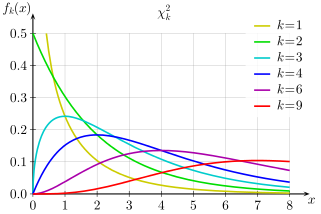
\includegraphics[scale=0.6]{x2dist.png}
  \end{minipage}
  \begin{minipage}[t]{3.5in}
    \begin{enumerate}
    \setlength{\itemsep}{5pt}
    \item[]
    \item If \(Z_i\iid\nd(0,1)\) then \(X=\sum Z_i^2\sim\Xs(k)\)
    \item \(E(X)=k\)
    \item \(V(X)=2k\)
    \end{enumerate}
  \end{minipage}
\end{properties}

\begin{theorem}
  Let \(X_i\iid\nd(\m,\o^2)\) such that \(\m\) and \(\o\) are unknown:
  \[\frac{(n-1)S^2}{\o^2}\sim\Xs(n-1)\]
\end{theorem}

\begin{theorem}
  Let \(X_i\iid\nd(\m,\o^2)\) such that \(\m\) and \(\o\) are unknown.  A \(1-\a\) confidence interval for \(\o^2\) is
  given by:
  \[\left(\frac{(n-1)s^2}{\xd{\frac{a}{2}}{n-1}},\frac{(n-1)s^2}{\xd{1-\frac{a}{2}}{n-1}}\right)\]
\end{theorem}

\begin{proof}
  \[P\left(a<\frac{(n-1)S^2}{\o^2}<b\right)=1-\a\]
  Let \(a=\xd{1-\frac{a}{2}}{n-1}\) and \(b=\xd{\frac{a}{2}}{n-1}\).
  \begin{gather*}
    P\left(\xd{1-\frac{a}{2}}{n-1}<\frac{(n-1)S^2}{\o^2}<\xd{\frac{a}{2}}{n-1}\right)=1-\a \\
    P\left(\frac{(n-1)S^2}{\xd{\frac{a}{2}}{n-1}}<\o^2<\frac{(n-1)S^2}{\xd{1-\frac{a}{2}}{n-1}}\right)=1-\a \\
  \end{gather*}
\end{proof}

\begin{example}
  A sample carton of brown eggs from a farm has \(s^2=4.69\).  Assuming a normal population with unknown variance, obtain a
  95\% confidence interval for \(\o^2\).
  \begin{gather*}
    1-\a=0.95 \\
    \a=1-0.95=0.05 \\
    \frac{\a}{2}=\frac{0.05}{2}=0.025 \\
    1-\frac{\a}{2}=1-0.025=0.975 \\
    \\
    \xd{0.025}{11}=21.920 \\
    \xd{0.975}{11}=3.816 \\
    \\
    (n-1)s^2=11(4.69)=51.59 \\
    \\
    \frac{(n-1)s^2}{\xd{\frac{a}{2}}{n-1}}=\frac{51.59}{21.92}\approx2.35 \\
    \frac{(n-1)s^2}{\xd{1-\frac{a}{2}}{n-1}}=\frac{51.59}{3.816}\approx13.52 \\
  \end{gather*}
  Thus, we are 95\% confident that the true value of \(\o^2\) is contained in \((2.35,13.52)\).
\end{example}

\end{document}
